%\documentstyle[epsf,twocolumn]{jarticle}       %LaTeX2e仕様
\documentclass[twocolumn]{jarticle}     %pLaTeX2e仕様(platex.exeの場合)
% \documentclass[onecolumn]{ujarticle}   %pLaTeX2e仕様(uplatex.exeの場合)
%%%%%%%%%%%%%%%%%%%%%%%%%%%%%%%%%%%%%%%%%%%%%%%%%%%%%%%%%%%%%%
%%
%%  基本バージョン
%%
%%%%%%%%%%%%%%%%%%%%%%%%%%%%%%%%%%%%%%%%%%%%%%%%%%%%%%%%%%%%%%%%
\setlength{\topmargin}{-45pt}
%\setlength{\oddsidemargin}{0cm}
\setlength{\oddsidemargin}{-7.5mm}
%\setlength{\evensidemargin}{0cm}
\setlength{\textheight}{24.1cm}
%setlength{\textheight}{25cm}
\setlength{\textwidth}{17.4cm}
%\setlength{\textwidth}{172mm}
\setlength{\columnsep}{11mm}

%\kanjiskip=.07zw plus.5pt minus.5pt


% 【節が変わるごとに (1.1)(1.2) … (2.1)(2.2) と数式番号をつけるとき】
%\makeatletter
%\renewcommand{\theequation}{%
%\thesection.\arabic{equation}} %\@addtoreset{equation}{section}
%\makeatother

%\renewcommand{\arraystretch}{0.95} 行間の設定
%%%%%%%%%%%%%%%%%%%%%%%%%%%%%%%%%%%%%%%%%%%%%%%%%%%%%%%%
%\usepackage{graphicx}   %pLaTeX2e仕様(\documentstyle ->\documentclass)
\usepackage[dvipdfmx]{graphicx}
\usepackage{subcaption}
\usepackage{multirow}
\usepackage{amsmath}
\usepackage{url}
\usepackage{ulem}
\usepackage{algorithm}
\usepackage{algorithmic}
\usepackage{listings} %,jlisting} %日本語のコメントアウトをする場合jlistingが必要
%ここからソースコードの表示に関する設定
\lstset{
  basicstyle={\ttfamily},
  identifierstyle={\small},
  commentstyle={\smallitshape},
  keywordstyle={\small\bfseries},
  ndkeywordstyle={\small},
  stringstyle={\small\ttfamily},
  frame={tb},
  breaklines=true,
  columns=[l]{fullflexible},
  numbers=left,
  xrightmargin=0zw,
  xleftmargin=3zw,
  numberstyle={\scriptsize},
  stepnumber=1,
  numbersep=1zw,
  lineskip=-0.5ex
}
%%%%%%%%%%%%%%%%%%%%%%%%%%%%%%%%%%%%%%%%%%%%%%%%%%%%%%%%
\begin{document}

	%bibtex用の設定
	%\bibliographystyle{ujarticle}

	\twocolumn[
		\noindent
		\hspace{1em}
		前期研究発表会資料 2022 年 7 月 6 日 (水)
		\hfill
	  M2 杉山 竜弥
		\vspace{2mm}

		\hrule
		\begin{center}
			{\Large \bf 手描きスケッチの類似度に基づく絵描き歌生成手法の検討}
		\end{center}
		\hrule
		\vspace{9mm}
	]

\section{はじめに}

% TODOs

% (要素技術)
% 原稿仕上げ
% みてもらう

% 授業
% 発表練習

  近年,機械学習の発展を背景に人工知能 (Artificial Intelligence : AI) が注目を浴びている.
  AI は単純なパターン認識では人間の能力を凌駕する性能を示す一方で,人間の情緒や感性に関する分野,特に人間の創作物への AI の適用はいまだ困難である.
  創作物の中でも,スケッチは,年齢,国籍,文化にかかわらず,幅広く共感可能な表現であるため重要度が高い.
  このため,感性を取り扱う分野での重要な AI の課題の 1 つとされてきた.
  また人工知能で画像データを扱う問題の場合,
  画像データの形式は画素の集合で高次元なラスタ形式のことが一般に多く,
  次元が少なく描き順の情報も持てるベクター形式での研究は多くない.

  本研究ではベクター形式のイラストのスケッチデータを用いて,
  創作物の 1 つである絵描き歌の生成を目指す.
  絵描き歌は画像,言語,音楽など様々なモーダルを含むため,
  極めて創作性を要する問題である.
  先行研究では単純なスケッチに対して,
  オブジェクトと位置関係を示す文章の生成に成功している.
  本研究では先行研究の手法を改良しより複雑なスケッチについて,
  絵描き歌らしい情緒的な歌詞を生成することを目標とし,
  改良したスケッチ分割手法を提案する.


\section{要素技術}

  \subsection{Sketch Recurrent Neural Network}	\label{tau}
    Sketch Recurrent Neural Network (Sketch RNN) \cite{sketchrnn} とは深層学習を用いて,人間がイラストを描くときの一連の描き順を学習することでユーザのイラストを補完,推測する深層学習を利用したモデルである.
    Sketch RNN の学習モデルは Variational Autoencoder (VAE) を基に構成されている.
    入力はスケッチの時系列を含む描き順を意味する行列であり,潜在ベクトルがエンコーダの出力となる.
    また,デコーダの出力は入力と同じ,画像を生成できる行列となる.

  \subsection{Accelerated KAZE}
  Accelerated KAZE (AKAZE) \cite{alcantarilla2011fast} は任意の画像に対して類似している画像を探す手法である.
  AKAZE は特徴点検出を行い画像の拡大や縮小回転に対して不変となっている KAZE をもとにしており,
  KAZE と同様に高い認識精度を持ちつつ計算に必要な時間を大幅に短縮している.
  類似度指標としては,マッチングした特徴点の距離平均を用いた.
  したがって 0 のとき完全に一致し,無関係のとき画像サイズに近くなる.

    \subsection{Cosine Similarity}
    コサイン類似度 (Cosine Similarity) は, 2 つのベクトルの類似性を表す尺度である.
    ベクトルがなす角がコサイン類似度となるため,1 のとき完全に類似し,0 のとき無関係となる.

    \begin{equation}
      \cos( \overrightarrow{a}, \overrightarrow{b} ) =
      \frac{\overrightarrow{a} \cdot \overrightarrow{b}}{|\overrightarrow{a}| |\overrightarrow{b}|}
    \end{equation}


	\subsection{Quick Draw データセット}
	Google が公開する描き順データセットである QuickDraw! \cite{Cheema:2012:QID:2207676.2208550} の形式を使用する.
	この形式では, 1 つの手描きスケッチを構成する描き順データは行列で保持される.
	描き順データの行方向は手描きスケッチの描き始めから描き終わりまでのペンの状態に関する情報を時系列に沿って保持する.
	また,描き順データの列方向はある時刻 $t$ におけるペンの状態を保持しており,$x$ 座標の相対値, $y$ 座標の相対値,ストロークの描き終わりのブール値をそれぞれベクトルで持っている.


\section{提案手法}

\subsection{絵描き歌生成}
% 藤井ら \cite{fujii} による
絵描き歌生成の先行研究 \cite{fujii} では
絵描き歌生成の問題を 3 つに分割していた.

まず「スケッチの類似度比較」では,
2 つのスケッチ同士の類似度を求める場合の適当な指標を定める.

次に「クラスラベル列の取得」では,
求めた類似度指標で 1 ストロークごとにデータベースと比較し,
最も近いクラスラベルの順列を取得する.

最後に「歌詞生成」では,
クラスラベルや位置情報から,
絵描き指示を生成的に構築していた.

本研究ではまず類似度指標を見直し,
スケッチデータで考えられる 2 つの途中経過と最終状態について,
新たにそれぞれを改良した指標を導入する.

また絵描き歌では一般に似ている別のオブジェクトを合成することで目的のスケッチを完成させるので,
2 つ目のクラスラベル列の取得についてスケッチの分割方法を改良する.
先行研究では 1 ストロークごとに分割していたが,
性能の向上のため意味のあるオブジェクトごとに分割する
新たなスケッチ分割手法を提案する.


\subsection{提案手法}
本研究では絵描き歌生成のために必要な「スケッチの類似度比較」と「スケッチの分割」
について 2 つの実験をした.
それぞれを実験 1,実験 2 とする.

実験 1 ではスケッチの類似度指標となる 3 つの候補について,
スケッチの類似度を比較しその結果を定性的に評価した.

実験 2 では実験 1 で求めた指標を用いて実際にスケッチを分割し,結果を比較した.


\section{実験 1 : スケッチの類似度}
% \subsection{目的}

\begin{figure*}[tb]
 \begin{minipage}{1\hsize}
 	\begin{center}
 		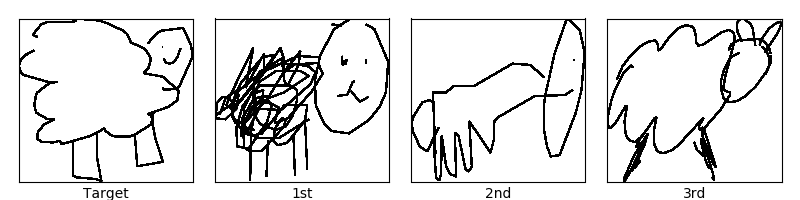
\includegraphics[clip,width=115mm]{sketch_trained_sim_A_0.png}
 		\caption{(手法A) Sketch RNN}
 		\label{fig:exp1_a}
 	\end{center}
 \end{minipage}

  \begin{minipage}{1\hsize}
  	\begin{center}
  		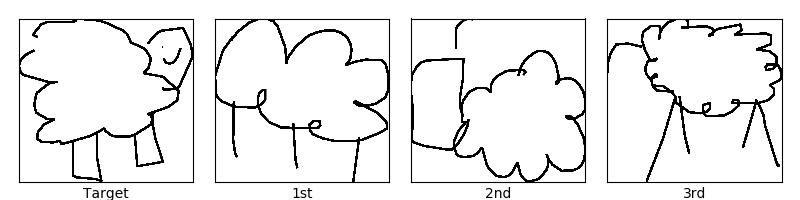
\includegraphics[clip,width=115mm]{sketch_trained_sim_B_0.png}
  		\caption{(手法B) AKAZE}
  		\label{fig:exp1_b}
  	\end{center}
  \end{minipage}

   \begin{minipage}{1\hsize}
   	\begin{center}
   		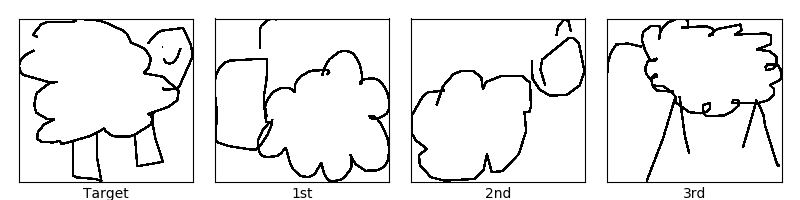
\includegraphics[clip,width=115mm]{sketch_trained_sim_D_0.png}
   		\caption{(手法C) Sketch RNN + AKAZE}
   		\label{fig:exp1_c}
   	\end{center}
   \end{minipage}
\end{figure*}

実験 1 では最適なスケッチの類似度指標を求める.
スケッチでは線を書く順番の「途中経過」と完成した「最終状態」を合わせた 2 つの状態があり,
この 2 つの状態を比較する必要がある.
この際に途中のストロークを考慮するか否かで 2 つの手法を用いる.

まず途中のストロークを考慮する場合はスケッチの時系列データを扱うことが出来る Sketch RNN を利用した.
Sketch RNN は Variational Autoencoder (VAE) であるため,
スケッチの時系列データを入力することで潜在ベクトル $z$ を得ることが出来る.
この $z$ のコサイン類似度を途中経過の類似度指標とした.
$S(x, y)$ を類似度関数, $E(x)$ をエンコーダとすると, $S_a$ は次式で表される.

\begin{equation}
  \label{equ:a}
  S_a(U, V) = \frac{E(U) \cdot E(V)}{|E(U)| |E(V)|}
\end{equation}


次に考慮しない場合はスケッチを画像化し,画像比較手法 AKAZE で比較した.
先行研究では画質評価手法 Structural Similarity (SSIM) が用いられていたが,
AKAZE は特徴点マッチングをするため画像の内容を比較できる.
AKAZE を用いた類似度 $S_b$ を

\begin{equation}
  \label{equ:b}
  S_b(U, V) = A \circ C_1 \circ \mathrm{Sigmoid} \circ C_2 (U, V)
\end{equation}

とした.
ここで $A$ は AKAZE 類似度, C は $S_a$ とスケールを合わせるための補正関数で, $C_1(x) = \frac{120 - x}{10}$, $C_2(x) = \frac{x + 1}{2}$ である.


これらを足し合わせ,途中経過と最終状態の両方を考慮する混合指標 $S_c$ を

\begin{equation}
  \label{equ:c}
  % S_c(U, V) = \frac{S_a(U, V) + S_b(U, V)}{2}
  S_c(U, V) = S_a(U, V) + S_b(U, V)
\end{equation}

とし,式 \ref{equ:a} ~ \ref{equ:c} でスケッチの類似度指標を評価する.

\subsection{実験設定}
スケッチデータセット QuickDraw から,対象とするスケッチとこれと比較するスケッチ 10 枚を取り出し,
3 つの類似度指標で実験した.
取り出したスケッチはいずれも "sheep" クラスである.

実験の設定は表 \ref{tab:setting1} に示す.
Sketch RNN のパラメータは事前に長時間学習したものを使用した.

\begin{table}[tb]
  \begin{center}
    \caption{Sketch RNN の設定}
    \begin{tabular}{cc} \hline
      \multicolumn{2}{c}{Parameter}  \\ \hline
      Learning step & 150,000 \\
      Learning rate & 0.001 \\
      Batch size & 100 \\
      Latent shape & (128, ) \\
      Decode temperature & 0.01 \\ \hline
    \end{tabular}
    \label{tab:setting1}
  \end{center}
\end{table}

\subsection{結果}
% A[(7, 0.9862899), (6, 0.89415294), (2, 0.7782751), (1, 0.57062423), (8, 0.4869256), (0, 0.0013451368), (3, -0.21240741), (9, -0.21476299), (5, -0.5499855), (4, -0.9028328)]
% B[(8, -116.04807692307692), (1, -116.8173076923077), (5, -118.45192307692308), (3, -120.98076923076923), (9, -121.09615384615384), (2, -121.10576923076923), (4, -122.03846153846153), (0, -130.45192307692307), (6, -131.46153846153845), (7, -131.46153846153845)]
% = [(8, 0.3675329896053509), (1, 0.3032792943562569), (5, 0.15298536646415564), (3, -0.09760859402959103), (9, -0.10896271676452136), (2, -0.10990703386698913), (4, -0.1997384988151555), (0, -0.7225552339045035), (6, -0.7535157530723093), (7, -0.7535157530723093)]

% C[(8, 1.0934066387256818), (5, 0.9155709468131241), (1, 0.2629781539584698), (6, 0.228598204332781), (7, 0.17851659365315453), (2, -0.05635251758133125), (3, -0.9260878840381359), (9, -1.0704136511746165), (4, -1.1764581166587835), (0, -1.580862833925866)]
% D[(1, 1.511369831256345), (4, 1.341358246262741), (5, 0.5409496028127758), (8, -0.017384995408811332), (9, -0.06231150135711422), (3, -0.1333689828363287), (2, -0.16729802033620456), (6, -0.6606084867923497), (0, -0.831266857121777), (7, -0.8643148704974889)]


図 \ref{fig:exp1_a}, \ref{fig:exp1_b}, \ref{fig:exp1_c} に実験 1 の結果を示す.
左から対象のスケッチと類似度が高いと判断された上位 3 つのスケッチである.

手法 A の Sketch RNN のみの場合は,描き順を考慮しているため最終状態は類似していない結果となった.
しかし胴体と頭,足を持った羊が右を向いていることから,描き順という点で評価すると妥当であると言える.

次に手法 B の AKAZE のみの場合は,羊毛の表現がなされているスケッチが選ばれており,
手法 A の場合と比較して極めて似ていることがわかる.
一方で体の部位や向きなどの描き順は無視されている.

最後に手法 C の両方を混合した指標は,AKAZE のみの手法 B と大きな変化はないが
 結果の上位 2 番目のスケッチはどちらか片方のみの場合ではなかったスケッチで,
 羊毛と体の向きも類似しており 比較がうまくいく場合もあることが確認された.


\section{実験 2 : スケッチの分割}

\begin{figure*}[tb]

 \begin{minipage}{1\hsize}
 	\begin{center}
 		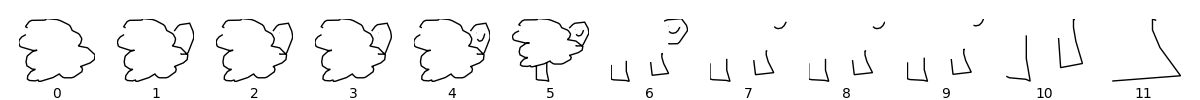
\includegraphics[clip,width=160mm]{origin.png}
 		\caption{分割候補となる部分スケッチ}
 		\label{fig:exp2_o}
 	\end{center}
 \end{minipage}
\vspace{2zh}

  \begin{minipage}{1\hsize}
  	\begin{center}
  		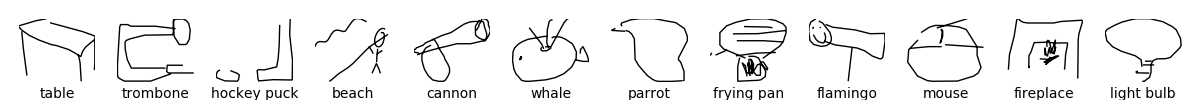
\includegraphics[clip,width=160mm]{sheep_a.png}
  		\caption{手法 A の Sketch RNN の推定結果}
  		\label{fig:exp2_a}
  	\end{center}
  \end{minipage}
 \vspace{1.5zh}

   \begin{minipage}{1\hsize}
     \begin{center}
       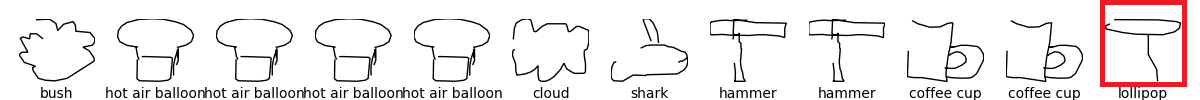
\includegraphics[clip,width=160mm]{sheep_b.png}
       \caption{手法 B の AKAZE の推定結果}
       \label{fig:exp2_b}
     \end{center}
   \end{minipage}
  \vspace{1.5zh}

    \begin{minipage}{1\hsize}
      \begin{center}
        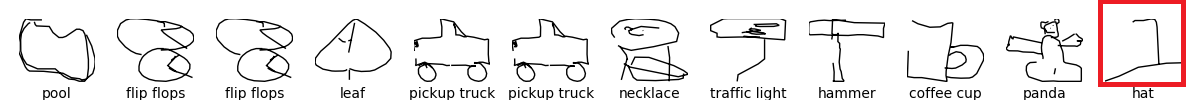
\includegraphics[clip,width=160mm]{sheep_c.png}
        \caption{手法 C の Sketch RNN + AKAZE の推定結果}
        \label{fig:exp2_c}
      \end{center}
    \end{minipage}

    \vspace{1zh}

\end{figure*}


実験 2 では実験 1 で求めた指標を用いて分割実験をした.
対象のスケッチに含まれる一部を取り出したものを「部分スケッチ」と呼ぶことにする.

実験 1 の 3 つの類似指標それぞれで,
部分スケッチに最も近い データベース中のクラスを求め,
対象のスケッチから最尤の部分スケッチのクラスラベルを得た.


\subsection{設定}
分割方法はスケッチのストローク列の中で 1 箇所を分割し, 2 つのスケッチに分けるように部分スケッチを得た.
したがって部分スケッチのストロークは順番が保たれる.

データベースの 345 クラスの代表スケッチ 1 枚から
最も類似度の高いものを部分スケッチの推定クラスとし,
全体で最大の類似度となった分割を求める.

実験 1 同様に "Sheep" クラスを分割対象として選んだ.
このスケッチは 7 画であるため,候補は 12 個となった.

\subsection{結果}

図 \ref{fig:exp2_o} ~ \ref{fig:exp2_c} に実験 2 の推定結果を示す.
図 \ref{fig:exp2_o} はストローク列の 1 箇所で分割される可能性がある部分スケッチの候補である.
図 \ref{fig:exp2_a} ~ \ref{fig:exp2_c} は各類似度におけるそれぞれの推定する類似スケッチとなる.
図の縦方向が各々の部分スケッチと 3 つの指標に対応している.
図の横方向で類似度最大となったクラススケッチは図中の赤枠で示す.


AKAZE 類似度を利用している手法の部分スケッチが一致した.
最も似ているのは Sketch RNN + AKAZE の"hat" クラスと思われる.
途中経過と最終状態を両方考慮することで,
類似度の性能が上がっている可能性がある.
定量的に評価するためアンケート調査を実施する予定である.

他の部分スケッチについてみると,
体を “bush” や “cloud” ,足を “coffee cup” と比較するなど
主観的に極めてマッチした推定結果もあったが,
これらが選ばれることはなかった.
このようなマッチしていると思われる部分スケッチが選ばれるように,
類似度指標の補正などの改良が必要であると考えられる.


\section{まとめと今後の課題}

書き順を含むスケッチデータに対して
絵描き歌生成のための新たな類似度指標と
スケッチの分割方法の提案をした.

類似度指標では,
AKAZE を用いた最終状態を入力する手法が良い結果となったが,
Sketch RNN のパラメータの性能が低かったことも原因として挙げられる.

スケッチの分割方法では,
先行研究ではなかったオブジェクトベースの視点を取り入れ,
一部では妥当な部分スケッチが得られた.

本研究では定性的な評価のみであったため,
定量的な評価としてアンケート調査をしたいと考えている.


今後の課題は本研究で得られたクラスラベルをもとに,
言語モデルを用いた絵描き歌の歌詞の生成をすることである.
また画像情報と言語情報がセットとなっているような
新たな絵描き歌用のデータセットを整備することが課題としてあげられる.

% 書き順を含むスケッチデータに対して~実験をし,類似度指標の考察をした.
%
% 絵描き歌用のデータセットを整備すること.
%
% 分割したクラスに対して言語モデルを通して,絵描き歌の歌詞を生成することが課題としてあげられる.
%
% ここにテキストを入力してください.ここにテキストを入力してください.ここにテキストを入力してください.ここにテキストを入力してください.ここにテキストを入力してください.ここにテキストを入力してください.ここにテキストを入力してください.ここにテキストを入力してください.

% 参考文献リスト
\bibliographystyle{unsrt}
\bibliography{ref}
\end{document}
